\documentclass{standalone}
\usepackage{tikz}
\usetikzlibrary{patterns, positioning}


\begin{document}
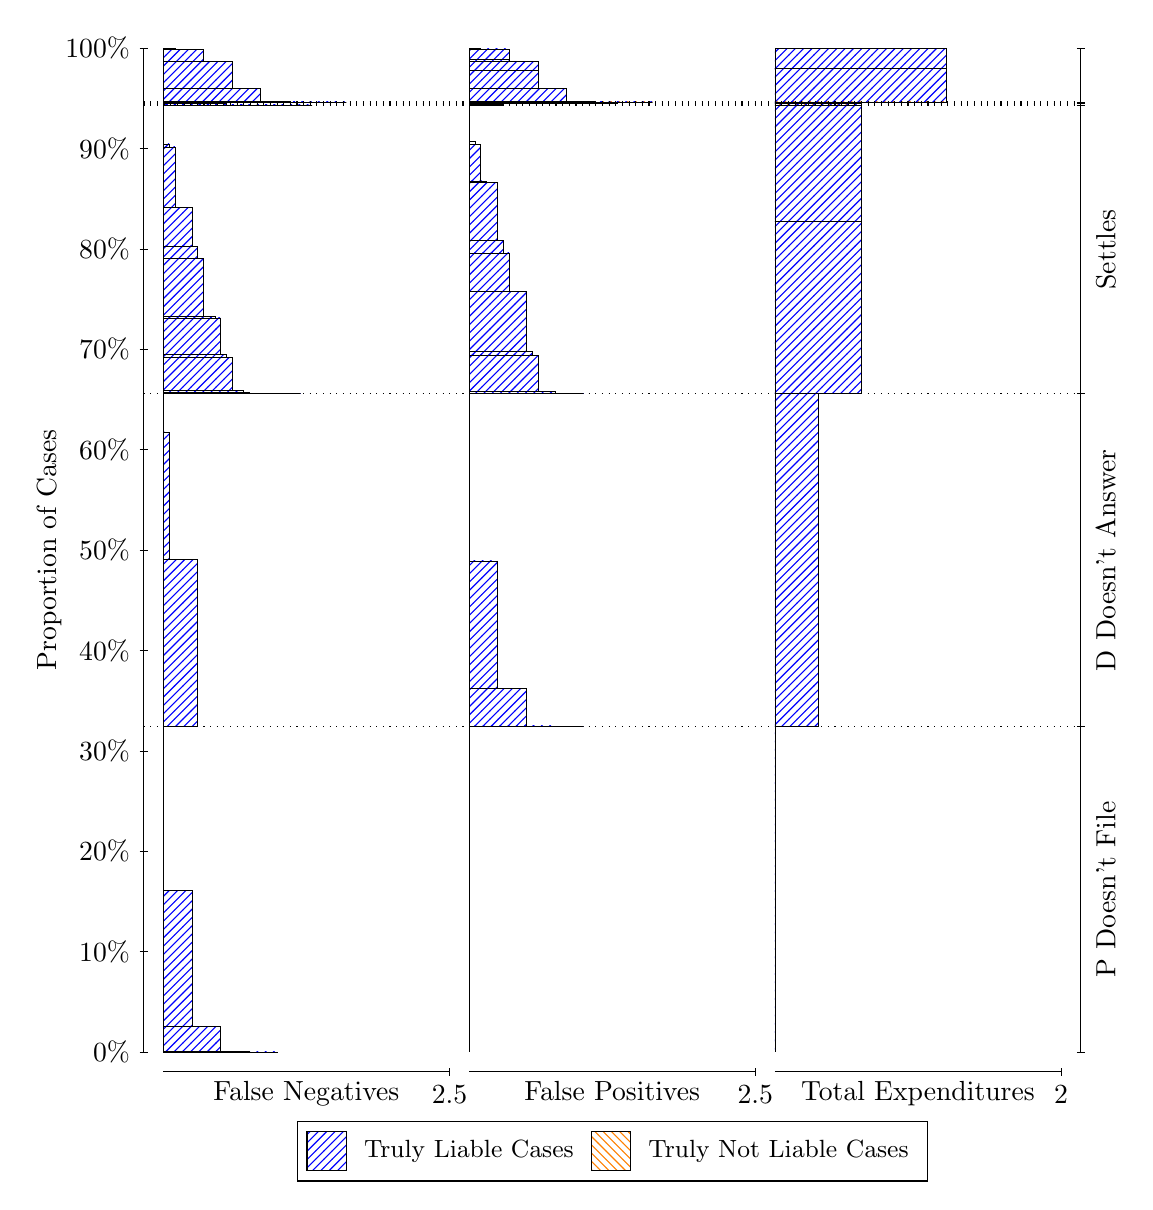
\begin{tikzpicture}
\draw[black, very thin] (1.5,1.75) -- (1.5,14.5);
\node[rotate=90, text=black, anchor=center] at (0.3, 8.125) {Proportion of Cases};
\draw[black, very thin] (1.45,1.75) -- (1.55,1.75);
\node[text=black, anchor=east] at (1.45, 1.75) {0\%};
\draw[black, very thin] (1.45,3.025) -- (1.55,3.025);
\node[text=black, anchor=east] at (1.45, 3.025) {10\%};
\draw[black, very thin] (1.45,4.3) -- (1.55,4.3);
\node[text=black, anchor=east] at (1.45, 4.3) {20\%};
\draw[black, very thin] (1.45,5.575) -- (1.55,5.575);
\node[text=black, anchor=east] at (1.45, 5.575) {30\%};
\draw[black, very thin] (1.45,6.85) -- (1.55,6.85);
\node[text=black, anchor=east] at (1.45, 6.85) {40\%};
\draw[black, very thin] (1.45,8.125) -- (1.55,8.125);
\node[text=black, anchor=east] at (1.45, 8.125) {50\%};
\draw[black, very thin] (1.45,9.4) -- (1.55,9.4);
\node[text=black, anchor=east] at (1.45, 9.4) {60\%};
\draw[black, very thin] (1.45,10.675) -- (1.55,10.675);
\node[text=black, anchor=east] at (1.45, 10.675) {70\%};
\draw[black, very thin] (1.45,11.95) -- (1.55,11.95);
\node[text=black, anchor=east] at (1.45, 11.95) {80\%};
\draw[black, very thin] (1.45,13.225) -- (1.55,13.225);
\node[text=black, anchor=east] at (1.45, 13.225) {90\%};
\draw[black, very thin] (1.45,14.5) -- (1.55,14.5);
\node[text=black, anchor=east] at (1.45, 14.5) {100\%};

\draw[black, very thin] (13.4,1.75) -- (13.4,14.5);
\draw[black, very thin] (13.35,1.75) -- (13.45,1.75);
\node[anchor=west] at (13.35, 1.75) {};
\draw[black, very thin] (13.35,5.8813) -- (13.45,5.8813);
\node[anchor=west] at (13.35, 5.8813) {};
\draw[black, very thin] (13.35,10.11) -- (13.45,10.11);
\node[anchor=west] at (13.35, 10.11) {};
\draw[black, very thin] (13.35,13.777) -- (13.45,13.777);
\node[anchor=west] at (13.35, 13.777) {};
\draw[black, very thin] (13.35,13.799) -- (13.45,13.799);
\node[anchor=west] at (13.35, 13.799) {};
\draw[black, very thin] (13.35,13.815) -- (13.45,13.815);
\node[anchor=west] at (13.35, 13.815) {};
\draw[black, very thin] (13.35,14.5) -- (13.45,14.5);
\node[anchor=west] at (13.35, 14.5) {};

\draw[black, very thin, pattern color=blue, pattern=north east lines] (1.75,1.75) rectangle (3.2033,1.75);
\draw[black, very thin, pattern color=blue, pattern=north east lines] (1.75,1.75) rectangle (2.84,1.7528);
\draw[black, very thin, pattern color=blue, pattern=north east lines] (1.75,1.7528) rectangle (2.4767,2.0776);
\draw[black, very thin, pattern color=blue, pattern=north east lines] (1.75,2.0776) rectangle (2.1133,3.8056);
\draw[black, very thin, pattern color=orange, pattern=north west lines] (1.75,3.8056) rectangle (1.75,3.8056);
\draw[black, very thin, pattern color=blue, pattern=north east lines] (1.75,3.8056) rectangle (1.75,5.8813);
\draw[black, very thin, pattern color=blue, pattern=north east lines] (1.75,5.8813) rectangle (2.186,8.0039);
\draw[black, very thin, pattern color=blue, pattern=north east lines] (1.75,8.0039) rectangle (1.8227,9.624);
\draw[black, very thin, pattern color=orange, pattern=north west lines] (1.75,9.624) rectangle (1.75,9.624);
\draw[black, very thin, pattern color=blue, pattern=north east lines] (1.75,9.624) rectangle (1.75,10.11);
\draw[black, very thin, pattern color=blue, pattern=north east lines] (1.75,10.11) rectangle (3.494,10.11);
\draw[black, very thin, pattern color=blue, pattern=north east lines] (1.75,10.11) rectangle (3.2033,10.11);
\draw[black, very thin, pattern color=blue, pattern=north east lines] (1.75,10.11) rectangle (3.1307,10.111);
\draw[black, very thin, pattern color=blue, pattern=north east lines] (1.75,10.111) rectangle (2.9127,10.112);
\draw[black, very thin, pattern color=blue, pattern=north east lines] (1.75,10.112) rectangle (2.84,10.129);
\draw[black, very thin, pattern color=blue, pattern=north east lines] (1.75,10.129) rectangle (2.7673,10.154);
\draw[black, very thin, pattern color=blue, pattern=north east lines] (1.75,10.154) rectangle (2.622,10.572);
\draw[black, very thin, pattern color=blue, pattern=north east lines] (1.75,10.572) rectangle (2.5493,10.614);
\draw[black, very thin, pattern color=blue, pattern=north east lines] (1.75,10.614) rectangle (2.4767,11.074);
\draw[black, very thin, pattern color=blue, pattern=north east lines] (1.75,11.074) rectangle (2.404,11.093);
\draw[black, very thin, pattern color=blue, pattern=north east lines] (1.75,11.093) rectangle (2.2587,11.832);
\draw[black, very thin, pattern color=blue, pattern=north east lines] (1.75,11.832) rectangle (2.186,11.988);
\draw[black, very thin, pattern color=blue, pattern=north east lines] (1.75,11.988) rectangle (2.1133,12.48);
\draw[black, very thin, pattern color=blue, pattern=north east lines] (1.75,12.48) rectangle (2.0407,12.48);
\draw[black, very thin, pattern color=blue, pattern=north east lines] (1.75,12.48) rectangle (1.8953,13.244);
\draw[black, very thin, pattern color=blue, pattern=north east lines] (1.75,13.244) rectangle (1.8227,13.283);
\draw[black, very thin, pattern color=orange, pattern=north west lines] (1.75,13.283) rectangle (1.75,13.283);
\draw[black, very thin, pattern color=blue, pattern=north east lines] (1.75,13.283) rectangle (1.75,13.777);
\draw[black, very thin, pattern color=blue, pattern=north east lines] (1.75,13.777) rectangle (3.6393,13.777);
\draw[black, very thin, pattern color=blue, pattern=north east lines] (1.75,13.777) rectangle (3.276,13.777);
\draw[black, very thin, pattern color=blue, pattern=north east lines] (1.75,13.777) rectangle (2.9127,13.778);
\draw[black, very thin, pattern color=blue, pattern=north east lines] (1.75,13.778) rectangle (2.5493,13.792);
\draw[black, very thin, pattern color=blue, pattern=north east lines] (1.75,13.792) rectangle (2.186,13.799);
\draw[black, very thin, pattern color=orange, pattern=north west lines] (1.75,13.799) rectangle (1.75,13.799);
\draw[black, very thin, pattern color=blue, pattern=north east lines] (1.75,13.799) rectangle (2.186,13.805);
\draw[black, very thin, pattern color=blue, pattern=north east lines] (1.75,13.805) rectangle (1.8227,13.814);
\draw[black, very thin, pattern color=orange, pattern=north west lines] (1.75,13.814) rectangle (1.75,13.814);
\draw[black, very thin, pattern color=blue, pattern=north east lines] (1.75,13.814) rectangle (1.75,13.815);
\draw[black, very thin, pattern color=blue, pattern=north east lines] (1.75,13.815) rectangle (4.0753,13.815);
\draw[black, very thin, pattern color=blue, pattern=north east lines] (1.75,13.815) rectangle (3.712,13.815);
\draw[black, very thin, pattern color=blue, pattern=north east lines] (1.75,13.815) rectangle (3.3487,13.825);
\draw[black, very thin, pattern color=blue, pattern=north east lines] (1.75,13.825) rectangle (2.9853,13.984);
\draw[black, very thin, pattern color=blue, pattern=north east lines] (1.75,13.984) rectangle (2.622,14.328);
\draw[black, very thin, pattern color=blue, pattern=north east lines] (1.75,14.328) rectangle (2.2587,14.487);
\draw[black, very thin, pattern color=blue, pattern=north east lines] (1.75,14.487) rectangle (1.8953,14.5);
\draw[black, very thin, pattern color=orange, pattern=north west lines] (1.75,14.5) rectangle (1.75,14.5);
\draw[black, very thin, pattern color=blue, pattern=north east lines] (1.75,14.5) rectangle (1.75,14.5);
\draw[black, very thin, pattern color=orange, pattern=north west lines] (5.6333,1.75) rectangle (5.6333,1.75);
\draw[black, very thin, pattern color=blue, pattern=north east lines] (5.6333,1.75) rectangle (5.6333,5.8813);
\draw[black, very thin, pattern color=orange, pattern=north west lines] (5.6333,5.8813) rectangle (7.0867,5.8813);
\draw[black, very thin, pattern color=blue, pattern=north east lines] (5.6333,5.8813) rectangle (7.0867,5.8813);
\draw[black, very thin, pattern color=blue, pattern=north east lines] (5.6333,5.8813) rectangle (6.7233,5.892);
\draw[black, very thin, pattern color=blue, pattern=north east lines] (5.6333,5.892) rectangle (6.36,6.3672);
\draw[black, very thin, pattern color=blue, pattern=north east lines] (5.6333,6.3672) rectangle (5.9967,7.9874);
\draw[black, very thin, pattern color=blue, pattern=north east lines] (5.6333,7.9874) rectangle (5.6333,10.11);
\draw[black, very thin, pattern color=orange, pattern=north west lines] (5.6333,10.11) rectangle (7.0867,10.11);
\draw[black, very thin, pattern color=blue, pattern=north east lines] (5.6333,10.11) rectangle (7.0867,10.11);
\draw[black, very thin, pattern color=orange, pattern=north west lines] (5.6333,10.11) rectangle (6.796,10.11);
\draw[black, very thin, pattern color=blue, pattern=north east lines] (5.6333,10.11) rectangle (6.796,10.111);
\draw[black, very thin, pattern color=blue, pattern=north east lines] (5.6333,10.111) rectangle (6.7233,10.14);
\draw[black, very thin, pattern color=orange, pattern=north west lines] (5.6333,10.14) rectangle (6.5053,10.14);
\draw[black, very thin, pattern color=blue, pattern=north east lines] (5.6333,10.14) rectangle (6.5053,10.604);
\draw[black, very thin, pattern color=blue, pattern=north east lines] (5.6333,10.604) rectangle (6.4327,10.643);
\draw[black, very thin, pattern color=blue, pattern=north east lines] (5.6333,10.643) rectangle (6.36,11.407);
\draw[black, very thin, pattern color=orange, pattern=north west lines] (5.6333,11.407) rectangle (6.2147,11.407);
\draw[black, very thin, pattern color=blue, pattern=north east lines] (5.6333,11.407) rectangle (6.2147,11.407);
\draw[black, very thin, pattern color=blue, pattern=north east lines] (5.6333,11.407) rectangle (6.142,11.899);
\draw[black, very thin, pattern color=blue, pattern=north east lines] (5.6333,11.899) rectangle (6.0693,12.054);
\draw[black, very thin, pattern color=blue, pattern=north east lines] (5.6333,12.054) rectangle (5.9967,12.794);
\draw[black, very thin, pattern color=blue, pattern=north east lines] (5.6333,12.794) rectangle (5.8513,12.813);
\draw[black, very thin, pattern color=blue, pattern=north east lines] (5.6333,12.813) rectangle (5.7787,13.273);
\draw[black, very thin, pattern color=blue, pattern=north east lines] (5.6333,13.273) rectangle (5.706,13.314);
\draw[black, very thin, pattern color=blue, pattern=north east lines] (5.6333,13.314) rectangle (5.6333,13.777);
\draw[black, very thin, pattern color=orange, pattern=north west lines] (5.6333,13.777) rectangle (6.0693,13.777);
\draw[black, very thin, pattern color=blue, pattern=north east lines] (5.6333,13.777) rectangle (6.0693,13.783);
\draw[black, very thin, pattern color=blue, pattern=north east lines] (5.6333,13.783) rectangle (5.706,13.798);
\draw[black, very thin, pattern color=blue, pattern=north east lines] (5.6333,13.798) rectangle (5.6333,13.799);
\draw[black, very thin, pattern color=orange, pattern=north west lines] (5.6333,13.799) rectangle (7.5227,13.799);
\draw[black, very thin, pattern color=blue, pattern=north east lines] (5.6333,13.799) rectangle (7.5227,13.799);
\draw[black, very thin, pattern color=blue, pattern=north east lines] (5.6333,13.799) rectangle (7.1593,13.799);
\draw[black, very thin, pattern color=blue, pattern=north east lines] (5.6333,13.799) rectangle (6.796,13.799);
\draw[black, very thin, pattern color=blue, pattern=north east lines] (5.6333,13.799) rectangle (6.4327,13.808);
\draw[black, very thin, pattern color=blue, pattern=north east lines] (5.6333,13.808) rectangle (6.0693,13.815);
\draw[black, very thin, pattern color=orange, pattern=north west lines] (5.6333,13.815) rectangle (7.9587,13.815);
\draw[black, very thin, pattern color=blue, pattern=north east lines] (5.6333,13.815) rectangle (7.9587,13.815);
\draw[black, very thin, pattern color=orange, pattern=north west lines] (5.6333,13.815) rectangle (7.5953,13.815);
\draw[black, very thin, pattern color=blue, pattern=north east lines] (5.6333,13.815) rectangle (7.5953,13.815);
\draw[black, very thin, pattern color=orange, pattern=north west lines] (5.6333,13.815) rectangle (7.232,13.815);
\draw[black, very thin, pattern color=blue, pattern=north east lines] (5.6333,13.815) rectangle (7.232,13.827);
\draw[black, very thin, pattern color=blue, pattern=north east lines] (5.6333,13.827) rectangle (6.8687,13.986);
\draw[black, very thin, pattern color=orange, pattern=north west lines] (5.6333,13.986) rectangle (6.8687,13.986);
\draw[black, very thin, pattern color=blue, pattern=north east lines] (5.6333,13.986) rectangle (6.8687,13.987);
\draw[black, very thin, pattern color=blue, pattern=north east lines] (5.6333,13.987) rectangle (6.5053,14.218);
\draw[black, very thin, pattern color=orange, pattern=north west lines] (5.6333,14.218) rectangle (6.5053,14.218);
\draw[black, very thin, pattern color=blue, pattern=north east lines] (5.6333,14.218) rectangle (6.5053,14.331);
\draw[black, very thin, pattern color=blue, pattern=north east lines] (5.6333,14.331) rectangle (6.142,14.359);
\draw[black, very thin, pattern color=blue, pattern=north east lines] (5.6333,14.359) rectangle (6.142,14.489);
\draw[black, very thin, pattern color=blue, pattern=north east lines] (5.6333,14.489) rectangle (5.7787,14.49);
\draw[black, very thin, pattern color=blue, pattern=north east lines] (5.6333,14.49) rectangle (5.7787,14.5);
\draw[black, very thin, pattern color=blue, pattern=north east lines] (5.6333,14.5) rectangle (5.6333,14.5);
\draw[black, very thin, pattern color=orange, pattern=north west lines] (9.5167,1.75) rectangle (9.5167,1.75);
\draw[black, very thin, pattern color=blue, pattern=north east lines] (9.5167,1.75) rectangle (9.5167,5.8813);
\draw[black, very thin, pattern color=orange, pattern=north west lines] (9.5167,5.8813) rectangle (10.062,5.8813);
\draw[black, very thin, pattern color=blue, pattern=north east lines] (9.5167,5.8813) rectangle (10.062,10.11);
\draw[black, very thin, pattern color=orange, pattern=north west lines] (9.5167,10.11) rectangle (10.607,10.11);
\draw[black, very thin, pattern color=blue, pattern=north east lines] (9.5167,10.11) rectangle (10.607,12.3);
\draw[black, very thin, pattern color=orange, pattern=north west lines] (9.5167,12.3) rectangle (10.607,12.3);
\draw[black, very thin, pattern color=blue, pattern=north east lines] (9.5167,12.3) rectangle (10.607,13.777);
\draw[black, very thin, pattern color=orange, pattern=north west lines] (9.5167,13.777) rectangle (10.607,13.777);
\draw[black, very thin, pattern color=blue, pattern=north east lines] (9.5167,13.777) rectangle (10.607,13.799);
\draw[black, very thin, pattern color=orange, pattern=north west lines] (9.5167,13.799) rectangle (10.607,13.799);
\draw[black, very thin, pattern color=blue, pattern=north east lines] (9.5167,13.799) rectangle (10.607,13.815);
\draw[black, very thin, pattern color=orange, pattern=north west lines] (9.5167,13.815) rectangle (11.697,13.815);
\draw[black, very thin, pattern color=blue, pattern=north east lines] (9.5167,13.815) rectangle (11.697,14.246);
\draw[black, very thin, pattern color=orange, pattern=north west lines] (9.5167,14.246) rectangle (11.697,14.246);
\draw[black, very thin, pattern color=blue, pattern=north east lines] (9.5167,14.246) rectangle (11.697,14.5);
\draw[black, dotted] (1.5,5.8813) -- (13.4,5.8813);
\draw[black, dotted] (1.5,10.11) -- (13.4,10.11);
\draw[black, dotted] (1.5,13.777) -- (13.4,13.777);
\draw[black, dotted] (1.5,13.799) -- (13.4,13.799);
\draw[black, dotted] (1.5,13.815) -- (13.4,13.815);
\draw[black, very thin] (1.75,1.5) -- (5.3833,1.5);
\node[text=black, anchor=north] at (3.5667, 1.5) {False Negatives};
\draw[black, very thin] (5.3833,1.45) -- (5.3833,1.55);
\node[text=black, anchor=north] at (5.3833, 1.45) {2.5};

\draw[black, very thin] (5.6333,1.5) -- (9.2667,1.5);
\node[text=black, anchor=north] at (7.45, 1.5) {False Positives};
\draw[black, very thin] (9.2667,1.45) -- (9.2667,1.55);
\node[text=black, anchor=north] at (9.2667, 1.45) {2.5};

\draw[black, very thin] (9.5167,1.5) -- (13.15,1.5);
\node[text=black, anchor=north] at (11.333, 1.5) {Total Expenditures};
\draw[black, very thin] (13.15,1.45) -- (13.15,1.55);
\node[text=black, anchor=north] at (13.15, 1.45) {2};

\node[text=black, centered, rotate=90] at (13.72, 3.8156) {P Doesn't File};
\node[text=black, centered, rotate=90] at (13.72, 7.9956) {D Doesn't Answer};
\node[text=black, centered, rotate=90] at (13.72, 11.943) {Settles};




\draw (7.449999999999999,1.5) node[draw=none] (baseCoordinate) {};
\begin{scope}[align=center]
        \matrix[scale=0.5, draw=black, below=0.5cm of baseCoordinate, nodes={draw}, column sep=0.1cm]{
            \node[rectangle, draw, minimum width=0.5cm, minimum height=0.5cm, pattern color=blue, pattern=north east lines] {}; &
            \node[draw=none, font=\small, text=black] (B) {Truly Liable Cases}; &
            \node[rectangle, draw, minimum width=0.5cm, minimum height=0.5cm, pattern color=orange, pattern=north west lines] {}; &
            \node[draw=none, font=\small, text=black] (B) {Truly Not Liable Cases}; \\
            };
\end{scope}

\end{tikzpicture}
\end{document}